\documentclass{article}
\usepackage{fancyhdr}
\usepackage[utf8]{inputenc}
\usepackage{graphicx}
\graphicspath{{images/}}
\usepackage{float}

\begin{document}

\begin{titlepage}
	\begin{center}
	\huge{University of Pretoria\\
	Software Engineering - COS 301}\\
	\line(1,0){400}\\
	\huge{\bfseries NavUp Software Requirements Specification}\\
	\line(1,0){200}\\
	Team Teal\\
	16 February 2017\\
	[3cm]
	\end{center}
	\begin{flushleft}
	\bfseries{Author(s):}
	\end{flushleft}
	\begin{flushleft}
	Tlaka Mankgwanyane	\hspace{10mm}{\textbf {u14351872}}\\
	Alberts Josef			\hspace{26mm}{\textbf{u14395283}}\\
	Oratile Motswagosele	\hspace{11mm}{\textbf{u15306195}}\\
	Carrim Muhammed		\hspace{14mm}{\textbf{u15019854}}\\
	Jackson Pearce			\hspace{22.5mm}{\textbf{u14044332}}\\
	Potgieter Linda		\hspace{21.6mm}{\textbf{u14070091}}\\
	Kanda Madimba			\hspace{19.5mm}{\textbf{u17289077}}\\
	\end{flushleft}
\end{titlepage}

\tableofcontents

\section{Introduction}
\subsection{Purpose} 
This is the system requirement specification (SRS) which aims to refine and expand on the required capabilities of the NavUP system.
This document includes discussions on the individual low coupled subsystems as well as functional and quality requirements. This SRS is intended for the developers of the NavUP system as well as the clients who own the system. It will refine what is required of the system, what the main purpose of the system will be and what additional capabilities it will have.
\subsection{Scope}
The system being designed will be able to guide a variety of users such as students, lecturers, and visitors through the University of Pretoria's (UP) various campuses. This system will be identified as the NavUP system, referencing the navigation it will provide to visitors of the UP campuses.\\\\
The system will be able to route users between buildings and on a campus, as well as guiding them to the chosen lecture hall within the building. Notifications will also be sent to the users through the application when he/she is near a venue where public events are currently or will in future take place. There will not be any notifications sent if the users is not near the venue where these events will occur. The user will be able to create a profile, which will unlock additional functionalities such as sharing locations with friends, saving frequently used places, and adding timetable integration.\\\\
The application will also be able to notify a user about high traffic areas which the user may want to avoid in order to arrive earlier at his/her destination. The system aims to simplify all users' navigation through the various UP campuses, ensuring quicker travel to destinations and avoidance of congested routes.
\subsection{Definitions, Acronyms, and Abbreviation}
SRS - System Requirement Specification\\
UP - University of Pretoria\\
NavUP - The system being designed, acronym for Navigate(Nav) University of Pretoria (UP).\\
System - The NavUp system that is being designed.\\
Product/Application - NavUP system\\
Traffic - Areas in which there is a higher concentration of users which may affect arrival times.\\
Hot Spots - Areas in which there are wi-fi access for the users.\\
PVT - Position, Velocity and Time.\\\\
\subsection{Overview}
This document will provide more details abut the product (NavUP), including different interfaces, memory requirements, operations, as well as site adaption requirements. Functions, characteristics, constraints, and dependencies will also be discussed. Lastly the document will elaborate on  the different requirements, including external interface and functional and performance requirements.

\section{Overall Description}
	\subsection{Product Perspective}
		\subsubsection{System Interfaces}
		The  main systems that the application will be interfacing with are the campus systems that collaborate with the application. These include the UP calender, UP Server and the on campus network infrastructure.
		\subsubsection{User Interfaces}
		There are not many user interfaces because they will mainly be interacting with their smartphones and not branching to any other platforms. However the application itself will have many interfaces for the user to use. These include the fitness screen, navigation screen as well as many others.
		\subsubsection{Hardware Interfaces}
		The application will run in tandem with the onsite campus wireless routers as well as utilising the smartphones GPS connection to satellites.
		\subsubsection{Software Interfaces}
		Software interfaces for the application will include many programming languages that will be used to create the application and to personalise based on a user’s preference.
	\subsection{Product Functions}
	This system would allow different user types to navigate around the University of Pretoria's main campus grounds.
	This system would include three different types of users, namely: a student; a staff member and a visitor. All three
	users of the system would be able search for specific buildings and receive a guided path from their current position 
	to the searched area. The student and staff member users would both be able to search for events happening on 
	the main campus grounds and be able to save their searched areas for quick searches in future use. The system
	will also have restricted areas so as not to lead users through restricted areas. Popular areas, such as the food court,
	will be ready to choose options making them easier and quicker to find. Emergency gathering areas will also be highlighted
	and highly visible to all users.
	\subsection{User Characteristics}
	There will be three user types, the student; the staff member and the visitor. All users will be able to access
	the basic functionalities of the system. They will be all be able to search for a location on the main campus 
	of University of Pretoria. \\\\
	A visitor user will be limited to searching for their conference or building that they
	require as the rest of the functionality will be of no interest to them.\\\\
	The student user will have access to basic finctionality of the system but will reeive push notifications of special events on
	campus such as a conference on the field of study or a club performing a showcase. This functionality will be 
	customizable for each user to choose the interests.\\\\
	The staff member user will receive basic access to the system along with routes to restricted areas, upcoming conference
	locations and special events on campus.
	\subsection{Constraints}
	The accuracy of this system will be limited as there is not Wi-Fi signal across the entire main campus. Most of the
	system's functionalities will be unavailable without internet access for the user. This is particularily problematic
	near the gates of the campus as the user will have to use their own internet connections.\\\\
	To detect the traffic density on campus, most people on campus will have to be connected and their location trcked.
	This becomes problematic when users are not connected as the traffic density will become inaccurate. Another potential
	problem with this is the strain the users will put on the system when many users are on campus simultaneously.\\\\
	This system will also rely on the University of Pretoia's calendar which require the calendar be up to date constantly.
	It will also require the organisers of conferences and showcases to input their respective events so that they can be showed 
	on the system. The problem here lies in that organisers may not input their events and so users will not become aware of them.
	\subsection{Assumptions and Dependencies}
	In order for this system to function properly we will have to make a few assumptions about the users on the system.
	Firstly we are assuming that every user has a smartphone or tablet capable of running this system readily available to them.
	We are also assuming that they will access to internet on a constant connection.\\\\
	We have also assumened that they are IT literate and thus able to make use of the system. This assumption is however
	neccesary in order to make this system.\\\\We are assuming that all users will remain connected to the system once on campus 		grounds for the detection of the traffic density calculations.\\\\
	This system will rely on several aspects being functional. It relies on the Wi-Fi routers being spread across campus
	grounds; that every user remains connected once on campus; that the hardware needed to run the system is in fact capable
	of doing so.\\\\This system also relies on users having adaquete devices capable of running the system. Another depencies is 		that the usersinput their interests so that relevant events are shown to them. \\\\
	The final assumption that we are making is that all university events as well as the university calendar is up to date so as to 
	correctly display only current events of the day.
\section{Specific Requirements}
	\subsection{External Interface Requirements}
		\subsubsection{System Interfaces}
The software’s system interface includes Wi-Fi networking, the system uses Wi-Fi access points for detecting locations both indoors and outdoors. 
The system also uses the campus map database for locating routes and site information, that is, building names, addresses, etc. 
Based on the GPS and campus map database, the system provides route guidelines to lecture halls, libraries and cafeterias. 
Other geographical information/data is read from the GPS.\\\\
GPS satellite broadcasts signals which are received by the GPS receiver, the GPS receiver processes the navigation equations 
to determine the users current PVT, that is, position, velocity, and time. Therefore, based on the user input, the system will start by validating 
the given input and determine the user’s current position, then from the user’s position the system should display the route guidelines to the destination.\\

	\subsubsection{User Interfaces}
The NavUp system will presents/launches the login page/form for users to login. The users should login to access more features, 
such as getting directions, calendar, etc. If for any reason the user is not registered or authenticated, the user should be able to 
register by using the “Sign-up” option. So, provided that the user has successfully logged-in, the user can search for locations within 
the campus. However, there might be many routes leading to the destination, so the user should have an option to choose an optimal 
route out of many available routes. There are different types of users, of which are students, visitors and lecturers.\newline
The NavUp system should have a "settings" option so that users can customize the application according to their needs.\\\\
The "settings" screen should display the user's options for application themes/colors, notification sounds, and fonts properties, etc.\\\\
Certain users have different roles, for example; students will most likely use the software to navigate to lecture halls and access academic calendars, 
but visitors will most likely use the software to navigate to offices and boardrooms or to find where their meetings are scheduled. 
Therefore, certain users will have different activities (based on their roles) available for use in the software (NavUp system).
 Therefore when the user inputs data, the system should communicate with the campus map database and the GPS to get locations and route guidelines.\\\\
The users, particularly students should have profiles/accounts where their recent searches and others activities can be stored. 
Therefore, the system should have an option for users to view their profiles, and that’s where they can see their search history or rather the most visited venue/location. \\

	\subsubsection{Hardware Interfaces}
Mobile phones and Wi-Fi routers are the primary hardware interfaces necessary for the NavUp system. The system should communicate
 with the Wi-Fi routers and make use of the Wi-Fi access points to determine routes and locations. The GPS will use broadcasted signals by 
the GPS satellites to get locations in real-time. \\

	\subsubsection{Software Interfaces}
The NavUp will run primarily on mobile phones (smart phones), therefore the application should be compatible across most, 
if not all ranges of mobile smart phones, that is, either the Android Operating System or the iOS. The NavUp system will make 
use of the Wi-Fi access points and GPS to determine the current location/position of the user both indoors and outdoors. The 
system will also use of web services to connect to the campus map database in order to determine routes and site information (building names, addresses, etc.). 
So, only the routes within the Hatfield campus are accessible and all the information is displayed in the system’s screen interface. 
The system will determine the current position of the user in real-time using the GPS. \\

	\subsubsection{Communication Interfaces}
{The system will frequently communicate with the map database and the GPS in order to determine 
locations and also get directions. The communication between the system and the campus map database is done through Wi-Fi access points and web services. 
The mobile Operating System handles all other internal communications for the systems’ performance and response time. 
The NavUp system should be more accurate as possible, that is to say, it shouldn’t necessarily detect the exact user’s location. 
However, it should be in range (within the radius of the user’s current location). When the system receives an input from the user, 
the system will communicate with the map database and the GPS to get locations and directions in real-time. The NavUp system should also allow 
for multiple users at the same time, this is to say, the system’s performance shouldn’t be proportional to the number of active users.} \\
	\subsection{Functional Requirements}
		\subsubsection{Types of Users}
			\begin{itemize}
				\item Students
				\begin{itemize}
					\item Undergrad
					\item Postgrad
				\end{itemize}
				
				\item Employees
				\begin{itemize}
					\item Lecturers
					\item Admin staff
					\item Internal constructors
				\end{itemize}
				
				\item Visitors
				\begin{itemize}
					\item Parents
					\item External constructors
					\item Prospective students
					\item Walk-ins
				\end{itemize}
				
				\item Administrators
				\begin{itemize}
					\item UP officials
					\item Student societies
					\item UP event management
				\end{itemize}
			\end{itemize}
		\subsubsection{Use Case Prioritization}
			\begin{itemize}
				\item Critical
					\begin{itemize}
						\item User identifies destination
						\item Application determines location
						\item A user must be able to see building names as he passes them
						\item A user must specify  the kind of access
						\item A user must be able to see the campus map without searching for a location
						\item Venues should be grouped into categories
							\begin{itemize}
							\item A user must select a destination from category without typing it out
							\end{itemize}
						\item A user must see all the routes o the venue
							\begin{itemize}
								\item Disabilities
								\item Avoiding pedestrian traffic congestion
							\end{itemize}
						\item The user must be able to see arrival time
					\end{itemize}
				\item Important
					\begin{itemize}
						\item The UP admin must be able to update venues
						\item The app must sync with the university calendar
						\item The events manager must be able to update events on the app
						\item Venues must be associated with events going to take place there
 						\item The UP student societies must be able to update their calendars on the app
						\item Log all activities
						\item Log user preferences
					\end{itemize}
				\item Nice To Have
					\begin{itemize}
						\item Fitness track
						\item A brief history about campus building as the user passes them
						\item Reward system if certain milestones archived
						
					\end{itemize}

			\end{itemize}
		
		\subsection{Use Cases And Actor-Interaction}
	\begin{center}
	\begin{itemize}
			\begin{figure}[H]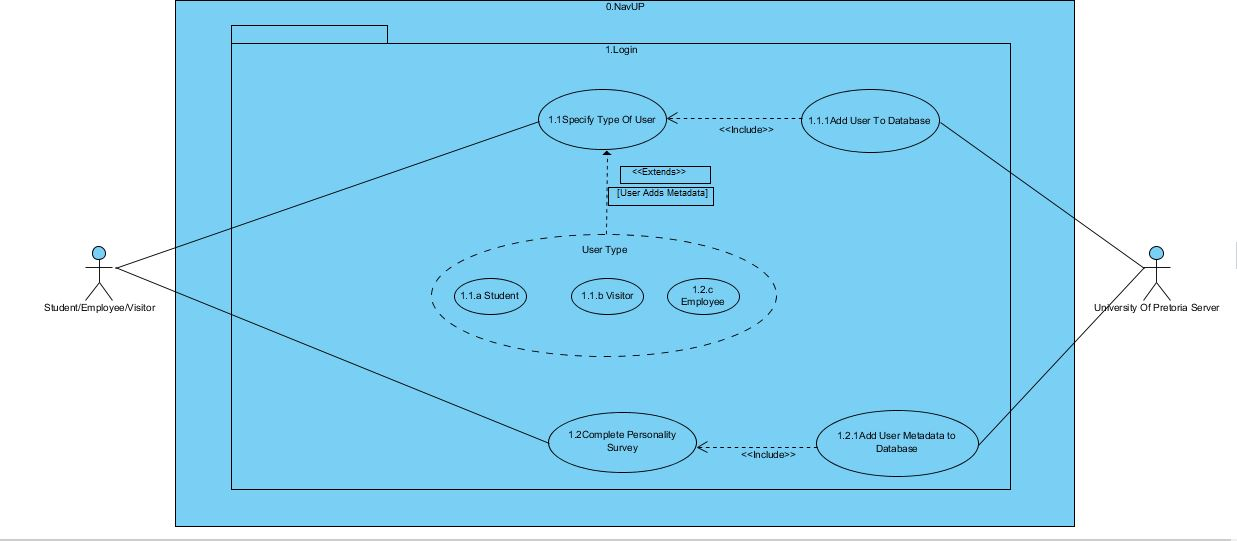
\includegraphics[width = \textwidth, height = 10cm]{Login.JPG} \end{figure}
			%\begin{flushleft}
			Figure 1: Login Use Case
			%\end{flushleft}
			\begin{figure}[H]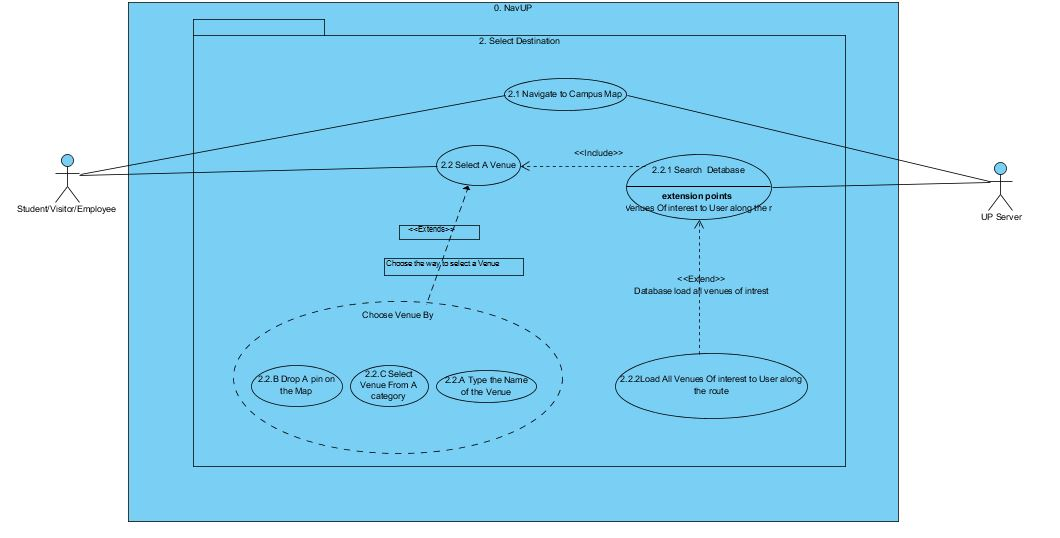
\includegraphics[width = \textwidth, height = 10cm]{Select_Destination.JPG} \end{figure}
			Figure 2: Select Destination Use Case
		%\item Figure 3: Route User
			\begin{figure}[H]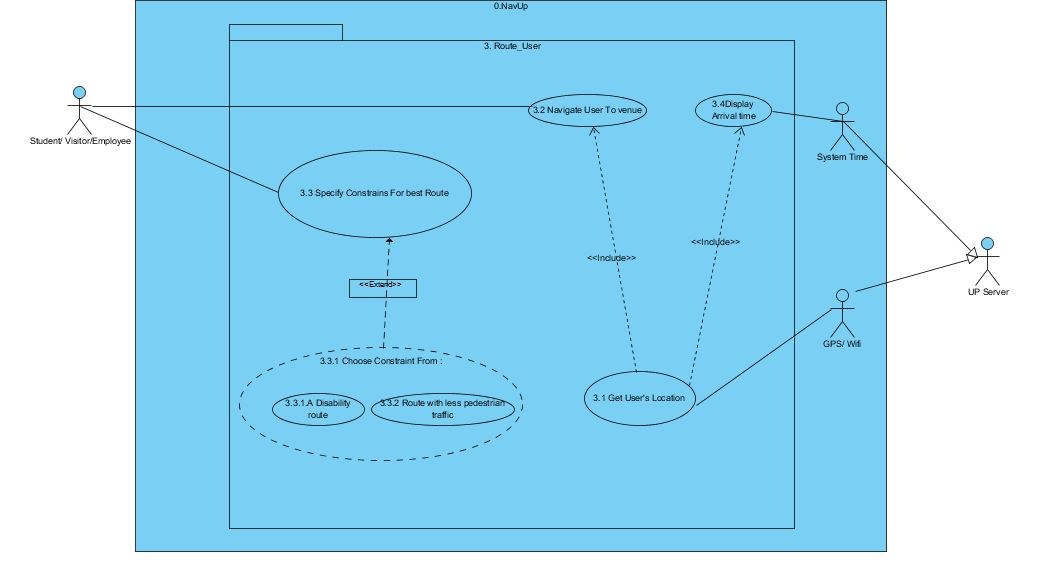
\includegraphics[width = \textwidth, height = 10cm]{Route_User.JPG} \end{figure}
			Figure 3: Route User Use Case
		%\item Figure 4: Login
			\begin{figure}[H]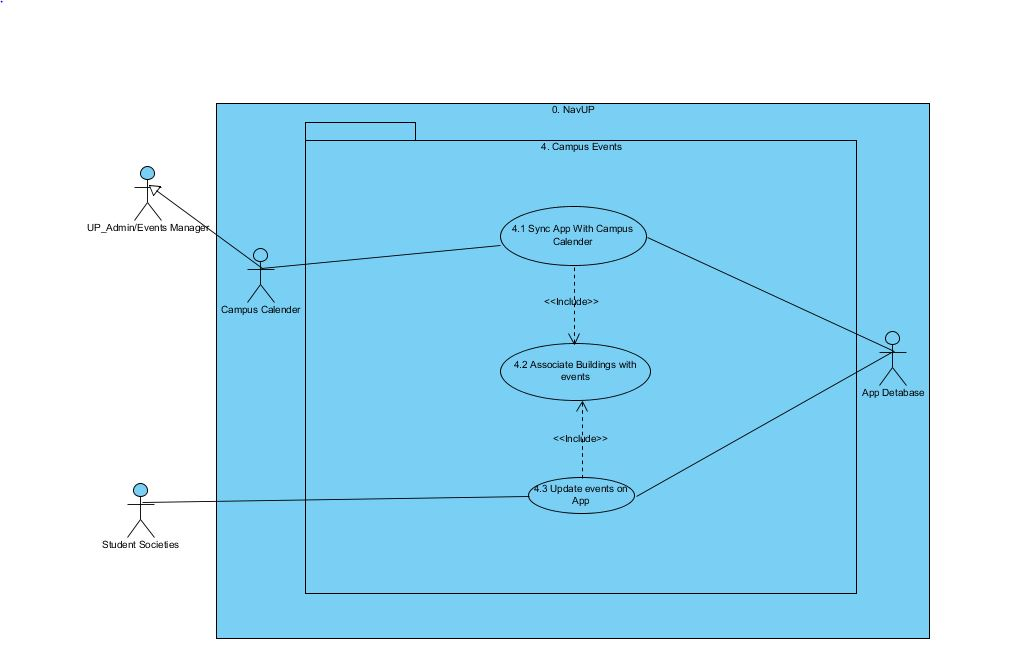
\includegraphics[width = \textwidth, height = 10cm]{Campus_Events.JPG} \end{figure}
			Figure 4: Campus Events Use Case
		%\item Figure 5: User fitness
			\begin{figure}[H]\includegraphics[width = \textwidth, height = 10cm]{User_fitness.JPG} \end{figure}
			Figure 5: User fitness Use Case

	\end{itemize}
	\end{center}
			\section{Test Cases}
			\subsection{Application Cold Start} %1.1
			\subsection{Application Warm Start} %1.2
			\subsection {Authentication} %1.3
			\subsection{Application Minimized} %1.4
			\subsection{Continuity} %1.5
			\subsection{Walk in Wrong Direction} %1.6
			\subsection{Traffic Congestion} %1.7
			\subsection{Accuracy} %1.8
			\subsection{Drawing Track} %1.9
			\subsection{Memory} %1.10
			\subsection{Computation Time} %1.11
			\subsection{Availability and Integrity (With Wi-Fi networking)} %1.12
\begin{flushleft}
\begin{tabular}{|c|c|c|c|c|c|c|c|c|c|c|c|c|c|}

\hline
 & \textbf{Test Cases} & 4.1 & 4.2 & 4.3 & 4.4 & 4.5 & 4.6 & 4.7 & 4.8 & 4.9 & 4.10 & 4.11 & 4.12 \\
\hline
\textbf{Req.} & & & & & & & & & & & & & \\
\hline
RQ1 UC1.1 & & & & X & & & & & & & & & \\
\hline
RQ1 UC1.2 & & & & X & X & X & & & & & & & \\
\hline
RQ2 UC2.1 &  & X & X & & & & &  & X & X & & & \\
\hline
RQ2 UC2.2 & & & & & & & & & X & X & & & \\
\hline
RQ2 UC2.2.1 & & & & & & & & & & & X & X & \\
\hline
RQ2 UC2.2.2 & & & & & X & & & X & X & X & & & \\
\hline
RQ3 UC3.1 & & & X & & & & & X & X & X & & & \\
\hline
RQ3 UC3.2 & & & & & & X & X & X & X & X & & & \\
\hline
RQ4 UC4.1 & & X & X & & & & & & & & & & X \\
\hline
RQ4 UC4.2 & & X & X & & & & & & X & & & & X \\
\hline
RQ4 UC4.3 & & & & & & & & & & & & & X \\
\hline
\end{tabular}
Figure 6: Requirement Traceability Matrix
\end{flushleft}	
	\subsection{Performance Requirements}
		\subsubsection{Position Accuracy} The position of a device with NavUP activated should be accurately determined by the system - with no more than 15m of deviation from actual location of the device.
		\subsubsection{Time to Determine Position} It should take NavUP no longer than 45 seconds to determine the location of the device (with reasonable accuracy) once the application has been opened.
		\subsubsection{Immidiacy of Push Notifications} Relevant push notifications should be pushed to the user's device no further than 30m from the focus of said notification. For example, current events at the AULA should not be displayed if a user is further than 30m from the AULA, to prevent cluttering of the notification bar.
		\subsubsection{View/Location Updates} Updates of the user's current location as displayed on the device screen should take place at intervals of no more than 5 seconds.
		\subsubsection{User Login} Upon providing the system with correct credentials, the application must present the user with the navigation screen within 7 seconds. 
	\subsection{Design Constraints}
		\subsubsection{Operating System/Platform} The system must be accessible from both Android and iOS devices - natively.		
	\subsection{Software System Attributes}
		\subsubsection{Reliability} The system should never cease working completely unless the error is caused by external systems outside our control (operating system, web APIs, etc). Decoupling should be such that modules, such as information on landmarks, should still be accessible if navigation fails. Ideally an entire system uptime (per month) of 99.9\% must be reached.
		\subsubsection{Maintainability} The system's code must be well documented, both by means of in-code comments and external documentation, to aid in maintaining the system.
		\subsubsection{Security \& Privacy} NavUP will allow user profiles to be created and personal information to be stored, no unauthorized users should have access to another user's information. Only administrators or the owner of the profile in question should have access to a profile's data.
		\subsubsection{Portability} The system must be available on both Android and iOS devices.
		\subsubsection{Scalability} It must be possible to scale the system backend in the event of an increase of users. Scaling must be possible both horizontally or vertically.
		\subsubsection{Response time} Following user interaction, the system may not delay more than 2 seconds before providing the user with feedback.
		\subsubsection{Usability} NavUP's core functions (navigation, news updates, suggestions) must be easy to understand and use. They must not take the average user more than a minute, each, to access and understand. 
\end{document}
